% Options for packages loaded elsewhere
\PassOptionsToPackage{unicode}{hyperref}
\PassOptionsToPackage{hyphens}{url}
%
\documentclass[
]{book}
\usepackage{lmodern}
\usepackage{amssymb,amsmath}
\usepackage{ifxetex,ifluatex}
\ifnum 0\ifxetex 1\fi\ifluatex 1\fi=0 % if pdftex
  \usepackage[T1]{fontenc}
  \usepackage[utf8]{inputenc}
  \usepackage{textcomp} % provide euro and other symbols
\else % if luatex or xetex
  \usepackage{unicode-math}
  \defaultfontfeatures{Scale=MatchLowercase}
  \defaultfontfeatures[\rmfamily]{Ligatures=TeX,Scale=1}
\fi
% Use upquote if available, for straight quotes in verbatim environments
\IfFileExists{upquote.sty}{\usepackage{upquote}}{}
\IfFileExists{microtype.sty}{% use microtype if available
  \usepackage[]{microtype}
  \UseMicrotypeSet[protrusion]{basicmath} % disable protrusion for tt fonts
}{}
\makeatletter
\@ifundefined{KOMAClassName}{% if non-KOMA class
  \IfFileExists{parskip.sty}{%
    \usepackage{parskip}
  }{% else
    \setlength{\parindent}{0pt}
    \setlength{\parskip}{6pt plus 2pt minus 1pt}}
}{% if KOMA class
  \KOMAoptions{parskip=half}}
\makeatother
\usepackage{xcolor}
\IfFileExists{xurl.sty}{\usepackage{xurl}}{} % add URL line breaks if available
\IfFileExists{bookmark.sty}{\usepackage{bookmark}}{\usepackage{hyperref}}
\hypersetup{
  pdftitle={Designcraft for experiments},
  pdfauthor={cjlortie},
  hidelinks,
  pdfcreator={LaTeX via pandoc}}
\urlstyle{same} % disable monospaced font for URLs
\usepackage{longtable,booktabs}
% Correct order of tables after \paragraph or \subparagraph
\usepackage{etoolbox}
\makeatletter
\patchcmd\longtable{\par}{\if@noskipsec\mbox{}\fi\par}{}{}
\makeatother
% Allow footnotes in longtable head/foot
\IfFileExists{footnotehyper.sty}{\usepackage{footnotehyper}}{\usepackage{footnote}}
\makesavenoteenv{longtable}
\usepackage{graphicx,grffile}
\makeatletter
\def\maxwidth{\ifdim\Gin@nat@width>\linewidth\linewidth\else\Gin@nat@width\fi}
\def\maxheight{\ifdim\Gin@nat@height>\textheight\textheight\else\Gin@nat@height\fi}
\makeatother
% Scale images if necessary, so that they will not overflow the page
% margins by default, and it is still possible to overwrite the defaults
% using explicit options in \includegraphics[width, height, ...]{}
\setkeys{Gin}{width=\maxwidth,height=\maxheight,keepaspectratio}
% Set default figure placement to htbp
\makeatletter
\def\fps@figure{htbp}
\makeatother
\setlength{\emergencystretch}{3em} % prevent overfull lines
\providecommand{\tightlist}{%
  \setlength{\itemsep}{0pt}\setlength{\parskip}{0pt}}
\setcounter{secnumdepth}{5}
\usepackage{booktabs}
\usepackage[]{natbib}
\bibliographystyle{apalike}

\title{Designcraft for experiments}
\author{cjlortie}
\date{2020-07-06}

\begin{document}
\maketitle

{
\setcounter{tocdepth}{1}
\tableofcontents
}
\hypertarget{introduction}{%
\chapter{Introduction}\label{introduction}}

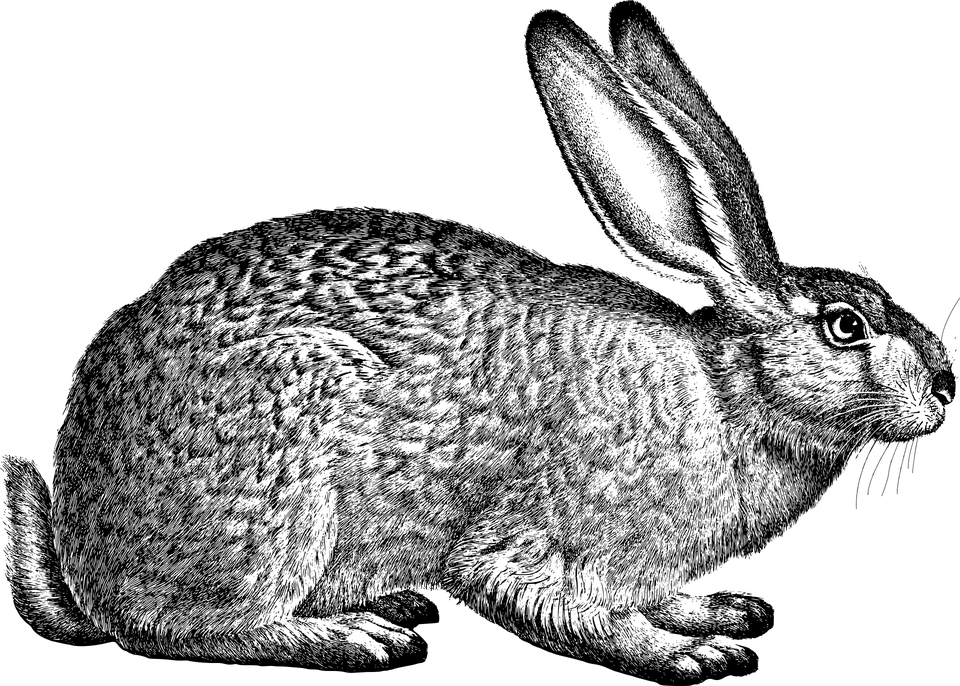
\includegraphics[width=4in,height=\textheight]{./rabbit.png}

Welcome to experimental design. There are two sets of three exercises provided to explore principles for better experiments. This is a simple book to support the practical, at-home learning associated with experimental design.

There are two primary modules. Field experiments comprises three outdoor experiments to explore sampling heterogeneous, complex processes in natural systems. The purpose is to provide choice. You need to try each, briefly, as a pilot experiment only. Then, select one to pursue in depth and write up. The data experiments describe the opportunity to use design thinking to structure existing data that others have already collected. The same principles for better experiments still apply in how you reuse the data. There are also three examples provided. Select only one and write up.

\hypertarget{gear-and-prep-for-field-experiments}{%
\subsubsection{Gear and prep for field experiments}\label{gear-and-prep-for-field-experiments}}

\hypertarget{prerequisites-for-data-experiment}{%
\subsubsection{Prerequisites for data experiment}\label{prerequisites-for-data-experiment}}

\hypertarget{birds}{%
\chapter{Balcony birdwatching}\label{birds}}

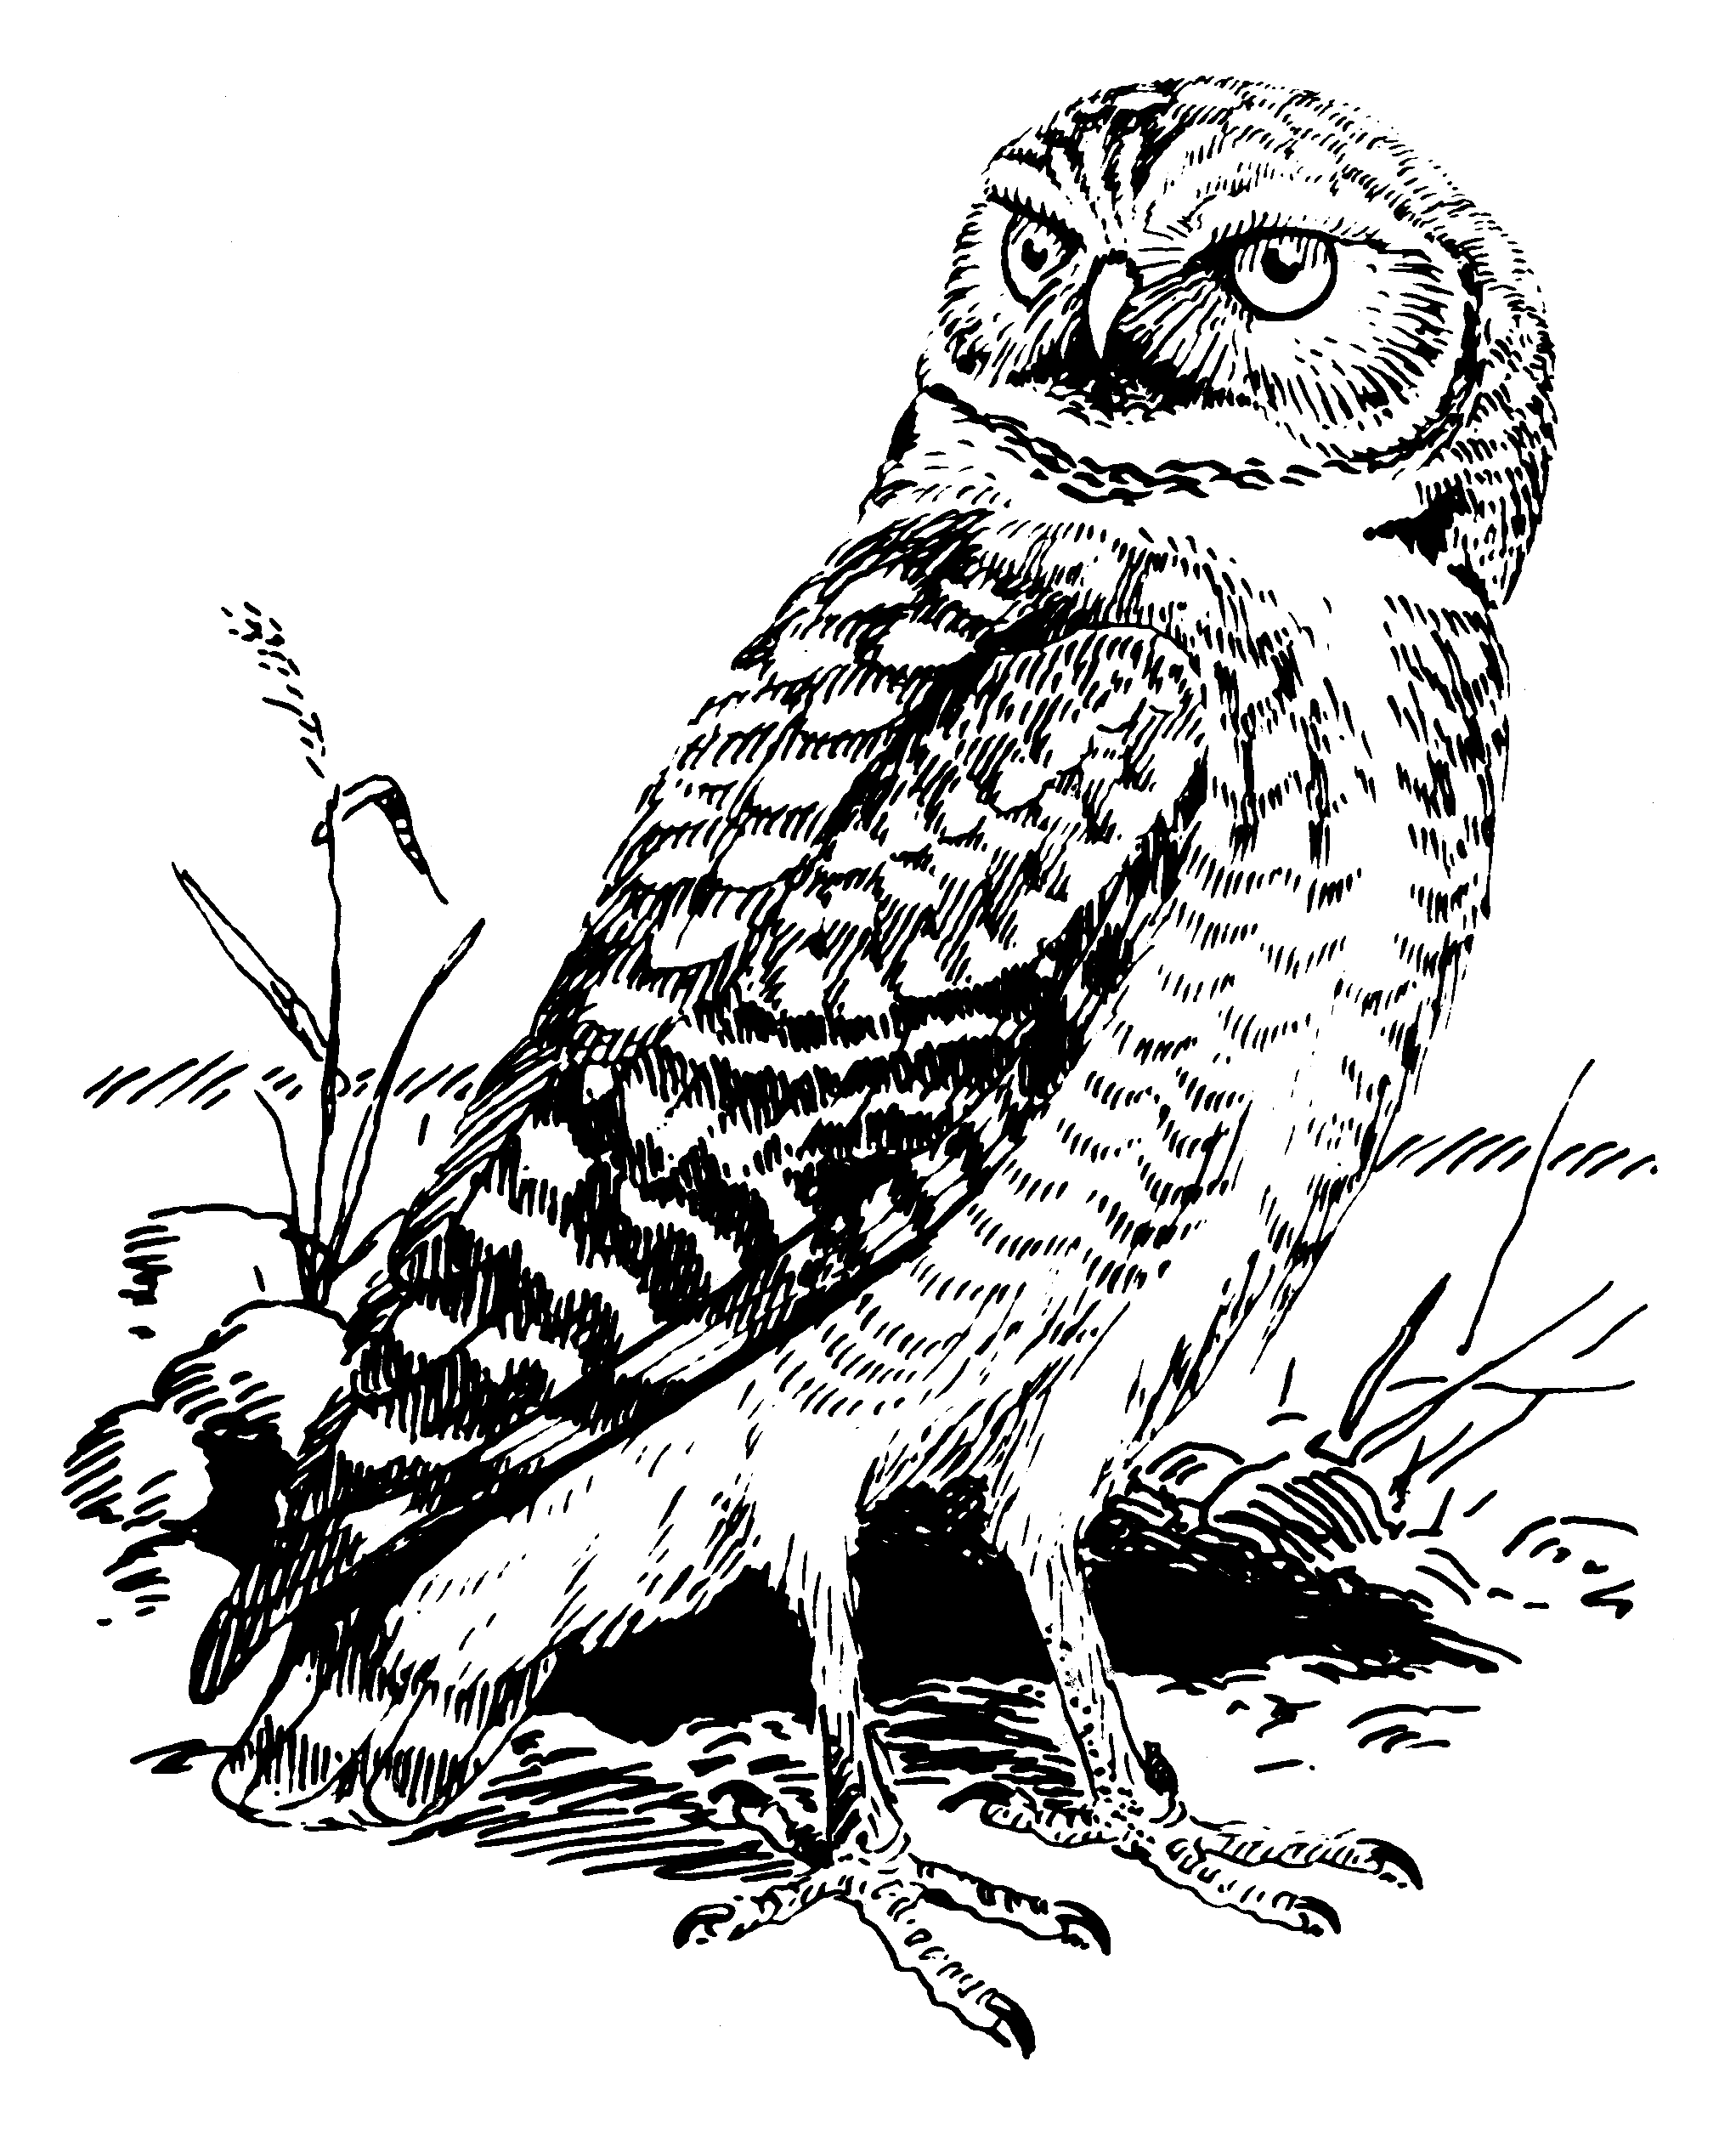
\includegraphics[width=4in,height=\textheight]{./owl.png}\\
Bird observation, from a distance.

\hypertarget{bioblitz}{%
\chapter{Backyard bioblitz}\label{bioblitz}}

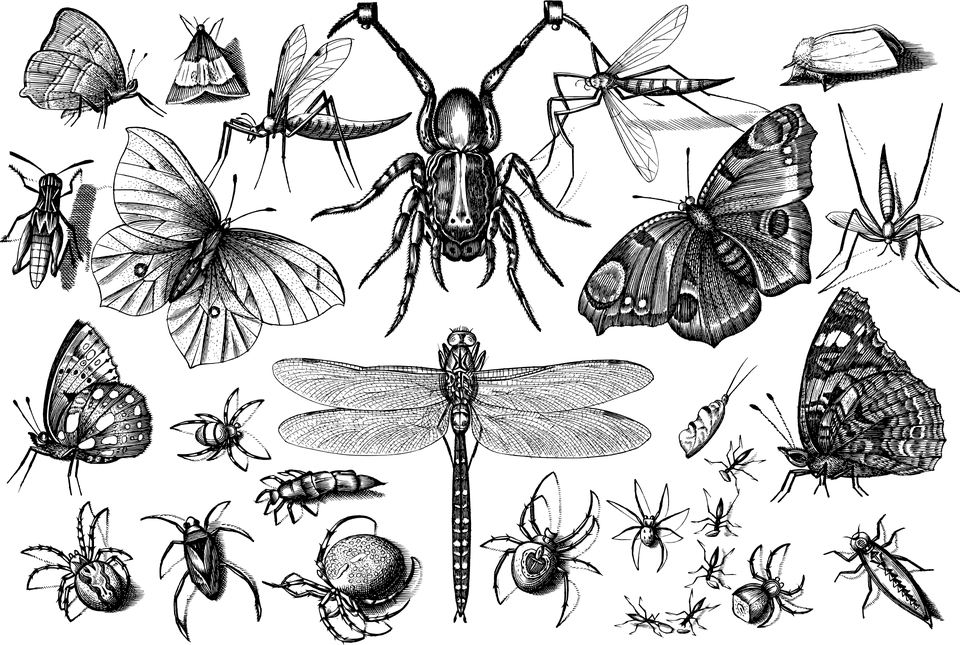
\includegraphics[width=4in,height=\textheight]{./insects.png}

A bioblitz is a biodiversity survey that is done rapidly for a specific place.

\hypertarget{survey}{%
\chapter{Solo surveys}\label{survey}}

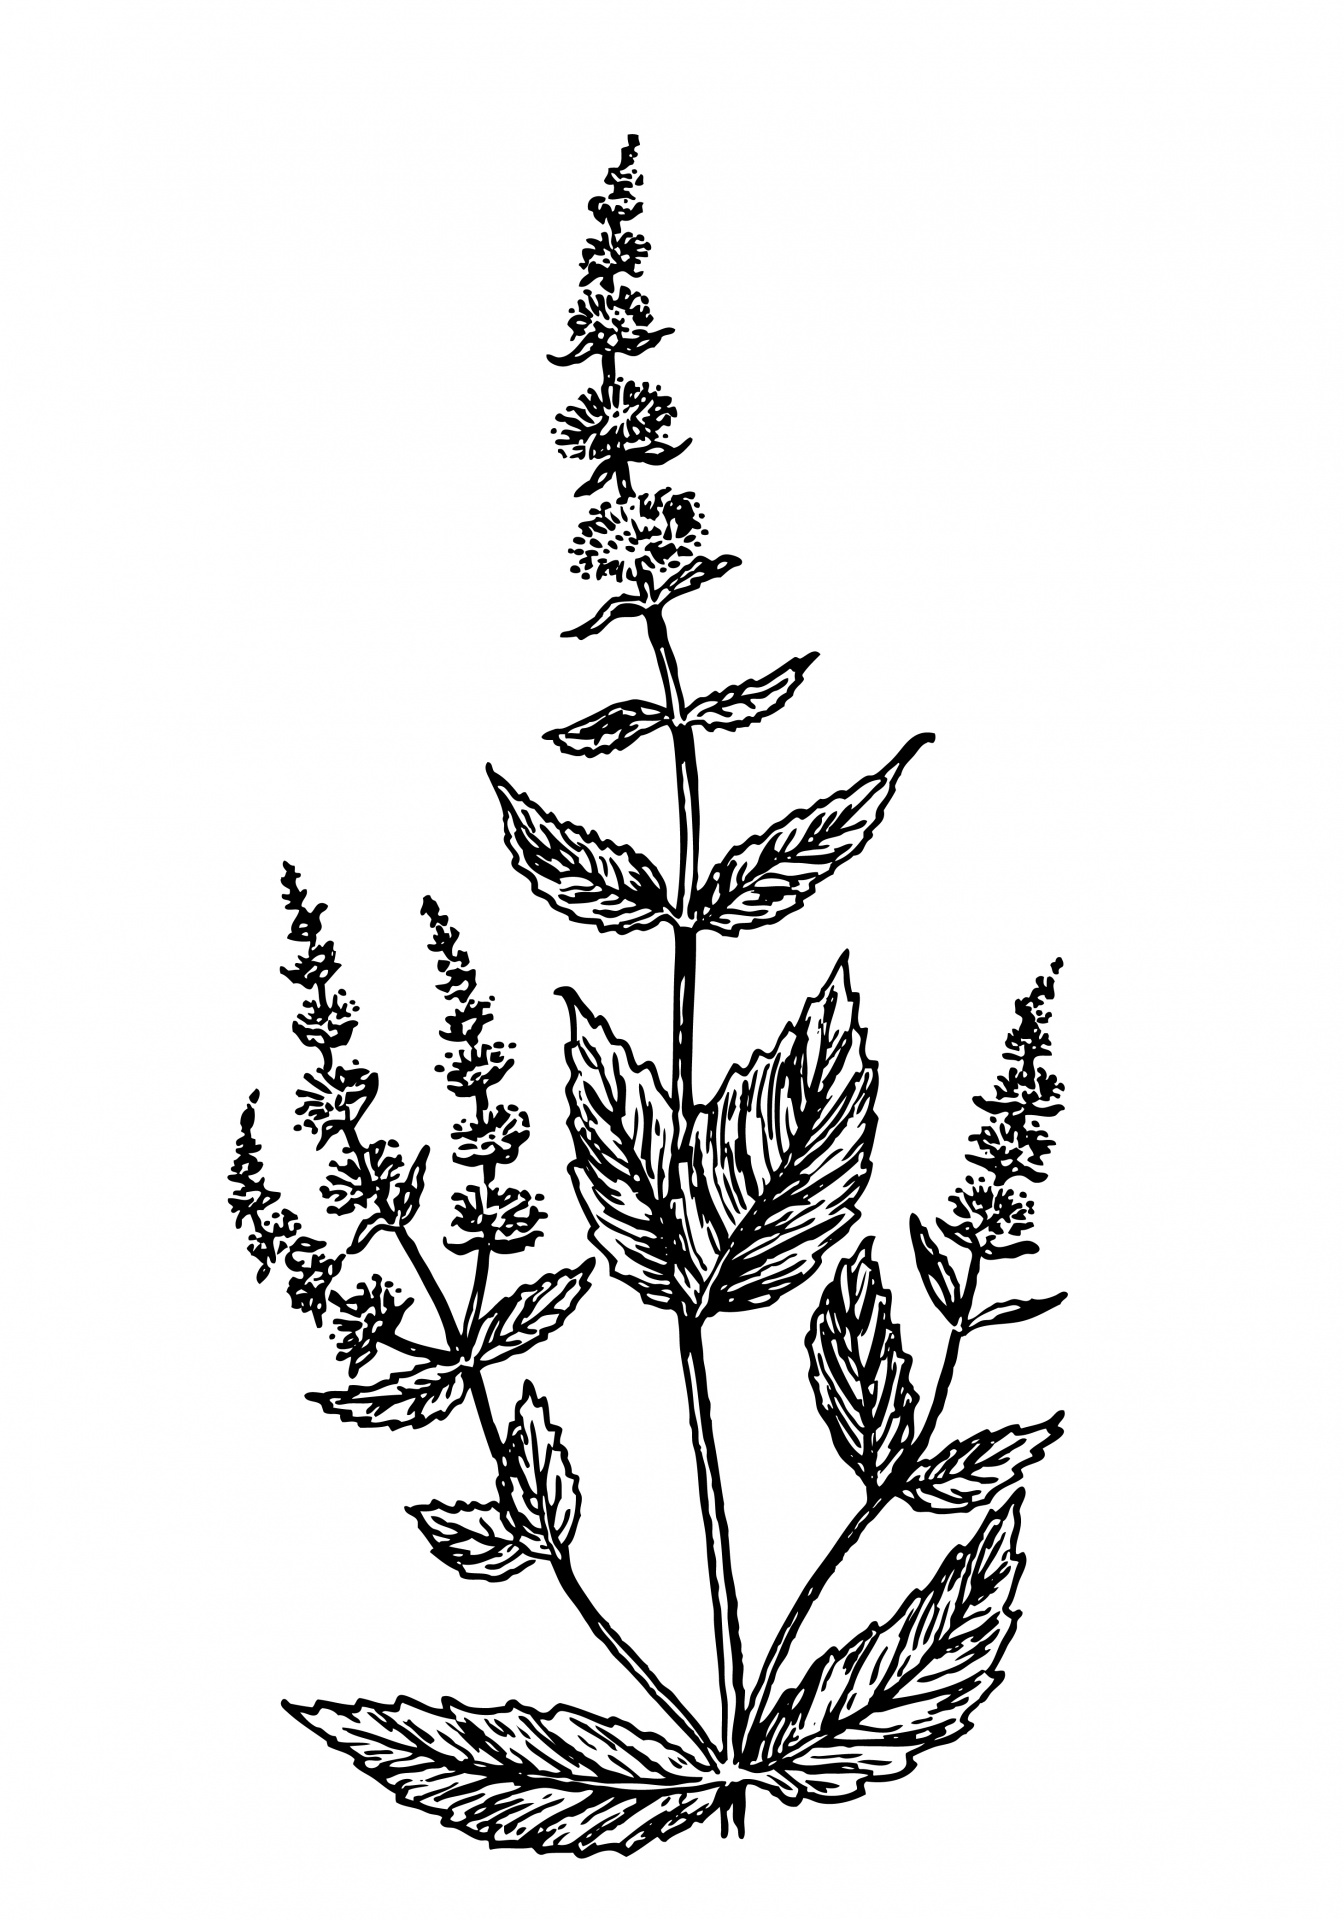
\includegraphics[width=4in,height=\textheight]{./plant.jpg}

Distributed ecological networks often use surveys done by individuals or small-teams to compile data on species or communities. Transects and quadrats are typically used to structure these `walk-through' surveys to estimate abundances and distributions of focal species.

\hypertarget{magic}{%
\chapter{Magic data}\label{magic}}

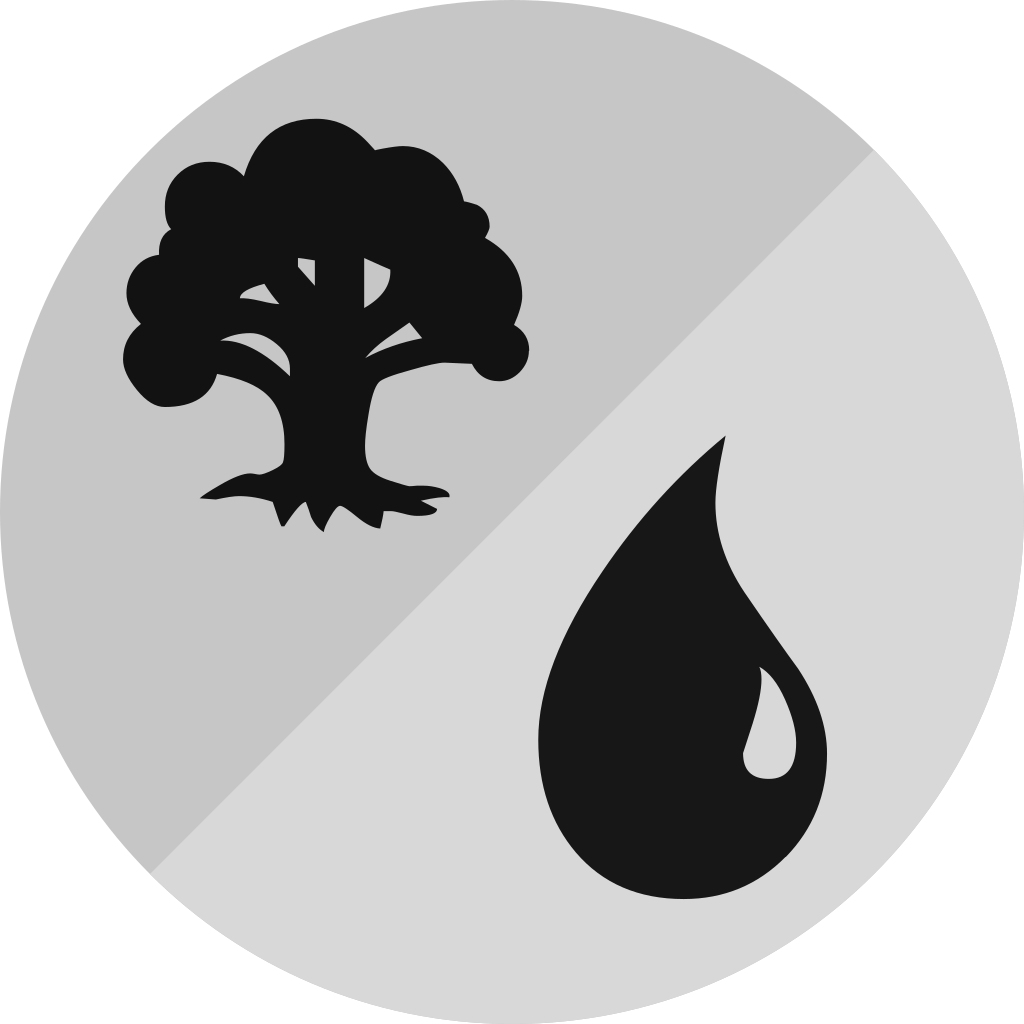
\includegraphics[width=4in,height=\textheight]{./magic.png}

Magic the Gathering is a popular collectible card game that includes strategy and chance.

\hypertarget{diversity}{%
\chapter{Diversity data}\label{diversity}}

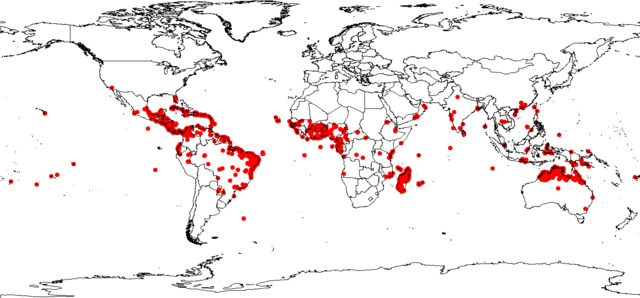
\includegraphics[width=4in,height=\textheight]{./gbif.png}

Diversity data from ebird or any citizen science project.

\hypertarget{humans}{%
\chapter{Human data}\label{humans}}

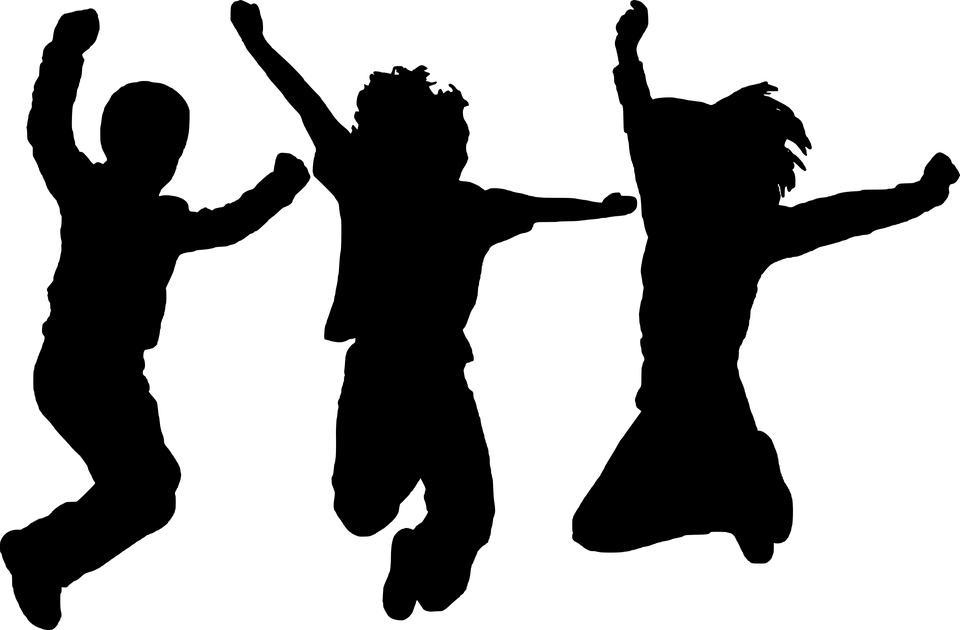
\includegraphics[width=4in,height=\textheight]{./humans.png}

Data associated with humans. Fitbit steps and sleep.

\hypertarget{notes}{%
\chapter{Final notes}\label{notes}}

Observations and conclusions.

  \bibliography{book.bib,packages.bib}

\end{document}
